\documentclass[english,a4paper,12pt]{report}
\usepackage{fancyhdr}
\usepackage{comment}
\usepackage{iftex}
\usepackage{graphicx}
\usepackage{geometry}
\usepackage{booktabs}
\usepackage{enumerate}
\usepackage{tabularx}
\usepackage{amsfonts}
\usepackage{blindtext}
\usepackage{qtree}
\usepackage{multicol}
\usepackage{amsmath,bm}
\usepackage{float}
\usepackage{amssymb}
\usepackage{wrapfig}
\restylefloat{figure}
\newcommand{\tabitem}{~~\llap{\textbullet}~~}
\usepackage{minted}
\usepackage{listings}
% \lstset{
%  basicstyle=\footnotesize,
%  language={[Objective]Caml},
%  breaklines=true,
%  tabsize=2,
%  frame=single,
%  numbers=left,
%  title=\lstname,
%  commentstyle=\color{mygreen},
%  numberstyle=\small\color{mygray},
%  stringstyle=\color{mymauve},
%  showstringspaces=false,
%  rulecolor=\color{black}
% }

\usepackage{xcolor}
\definecolor{codegreen}{rgb}{0,0.6,0}
\definecolor{codegray}{rgb}{0.5,0.5,0.5}
\definecolor{codepurple}{rgb}{0.58,0,0.82}
\definecolor{backcolour}{rgb}{0.95,0.95,0.92}
%Code listing style named "mystyle"

\usepackage{color}
\usepackage[draft=false]{hyperref}
\hypersetup{
    colorlinks=true, % make the links colored
    linkcolor=blue, % color TOC links in blue
    urlcolor=blue, % color URLs in blue
    linktoc=all % 'all' will create links for everything in the TOC
}
    
\urlstyle{same}
\lstdefinestyle{mystyle}{
  backgroundcolor=\color{backcolour},   commentstyle=\color{codegreen},
  keywordstyle=\color{magenta},
  numberstyle=\tiny\color{codegray},
  stringstyle=\color{codepurple},
  basicstyle=\ttfamily\footnotesize,
  breakatwhitespace=false,         
  breaklines=true,                 
  captionpos=b,     
  upquote=true,
  keepspaces=true,                 
  numbers=left,                    
  numbersep=5pt,                  
  showspaces=false,                
  showstringspaces=false,
  showtabs=false,                  
  tabsize=2
}


%"mystyle" code listing set
\lstset{style=mystyle}
\geometry{verbose,tmargin=4cm,bmargin=4cm,lmargin=1.5cm,rmargin=1cm,headheight=2.7cm,headsep=1cm,footskip=2cm}
\usepackage{array}
%
\def \hsp {\hspace{3mm}}
%
\makeatletter
\providecommand{\tabularnewline}{\\}
\makeatother
%
\ifxetex
\usepackage[T1]{fontenc}
\usepackage{fontspec}
\newfontfamily\nakulafont[AutoFakeBold=2]{Nakula}
\newfontfamily\liberationfont{Liberation Sans Narrow}
\newfontfamily\liberationsansfont{Liberation Sans}
\fi
%
\usepackage{tikz}
\usepackage{xcolor}
%
% 
\definecolor{circleorange}{rgb}{1,0.17,0.08}
\definecolor{darkorange}{rgb}{1,0.27,0.1}
\definecolor{orange2}{rgb}{1,0.5,0.15}
\definecolor{orange3}{rgb}{1,0.65,0.25}
\definecolor{yellow1}{rgb}{0.95,0.77,0.2}
\newcommand{\Omit}[1]{}
\fancypagestyle{plain}{
  \fancyhead[LO]
  {
\textbf{Compilers-II} \newline 
\textbf {Indian Institute of Technology Hyderabad \newline
Final Report \newline
Stoichy}\newline
	  }
	  
%
	  \fancyhf[ROH]{

\begin{tikzpicture}[scale=0.25,every node/.style={transform shape}]
\draw [fill=circleorange,circleorange] (5,10) circle (1.15); 
\fill [darkorange] (5.06,8) -- (5.06,2) -- (7.3,1.2) -- (7.3,8.8) -- (5.06,8);
\fill [darkorange] (4.94,8) -- (4.94,2) -- (2.7,1.2) -- (2.7,8.8) -- (4.94,8);
\fill [orange2]    (7.4,8.4) -- (7.4,1.6) -- (8.2,1.2) -- (8.2,8.8) -- (7.4,8.4);
\fill [orange2]    (2.6,8.4) -- (2.6,1.6) -- (1.8,1.2) -- (1.8,8.8) -- (2.6,8.4);
\fill [orange3]    (8.3,8.4) -- (8.3,1.6) -- (9.0,1.2) -- (9.0,8.8) -- (8.3,8.4);
\fill [orange3]    (1.7,8.4) -- (1.7,1.6) -- (1.0,1.2) -- (1.0,8.8) -- (1.7,8.4);
\fill [yellow1]    (9.1,8.4) -- (9.1,1.6) -- (9.7,1.2) -- (9.7,8.8) -- (9.1,8.4);
\fill [yellow1]    (0.9,8.4) -- (0.9,1.6) -- (0.3,1.2) -- (0.3,8.8) -- (0.9,8.4);
\ifxetex
\node [scale=2.1] at (5,-0.1)  {   {\bf {\nakulafont  भारतीय प्रौद्योगिकी संस्थान हैदराबाद }} };
\node [scale=1.8] at (5,-1.2) {   {\bf {\liberationsansfont Indian Institute of Technology Hyderabad}} };
\fi
\end{tikzpicture}
		  }
%
\renewcommand\headrule
 {

\begin{tikzpicture}
\definecolor{yellow1}{rgb}{0.95,0.77,0.2}
\draw[line width=0.75mm, yellow1] (0,0) -- (\textwidth,0);
\end{tikzpicture} 
 }}
 \pagestyle{plain}


\title{\textbf{\underline{\Huge{Stoichy}}}\\~\\
\textbf{Final Report }\\ 
Professor Ramakrishna Upadrasta\\
}
\author{K Vamshi  \and  Akash Tadwai  \and Vinta Reethu \and Havya K  \and Sai Varshittha }
\date{\today}
\usepackage{titlesec}

\begin{document}
\titleformat{\chapter}[display]   
{\normalfont\huge\bfseries}{\chaptertitlename\ \thechapter}{20pt}{\Huge}   
\titlespacing*{\chapter}{0pt}{-10pt}{40pt}
\maketitle

\tableofcontents
  
\chapter*{Introduction}
\addcontentsline{toc}{chapter}{Introduction}
     \textbf{\textit{Stoichy}} is a language that can be used to solve problems in different fields of chemistry , like stoichiometric calculations, oxidation-reduction reactions, acid-base reactions, thermodynamics, and electrochemistry. The questions in chemistry are generally procedural and there’s a common approach to understand each specific type of issue. \newline 
     For example, to find the molar mass of a molecule, we use the molar mass of an element and the number of moles of each element present in 1 mole of the compound and based on this info, we then calculate the mass of 1 mole of the compound. \vspace{1cm}
     Sometimes, these calculations become very complex to be done by hand, lets say, where we need to balance an equation with consisting many elements and complex compounds, where we need to solve for many variables using linear equations. All these kind of problems can generally be solved in a unique stepwise procedure involving calculations, solving linear equations,etc, which can even be applied to complex models and equations too.\\\\
    Solving all such problems can be done simply by using Stoichy, where we use data types and functions that are explictly designed to suit such needs, handles all such complex calculations and users can save a lot of time by making use of this language. \\\\We have implemented this by using a multi-paradigm   language Ocaml by using it's functional features. 
\newpage
\chapter{Language Tutorial}
\section{Pre-requisites}
The whole project needs \textbf{java} and some other libraries. First one need to install java and then run the bash script \textbf{prereqs.sh} in \textbf{sudo} mode to install all dependenices.
\section{Program Execution }
We have written a \textit{make} file, which on compiling would give an executable file named \textbf{stoichy}. The extension for our language is \textbf{sthy}, in order to compile a .sthy file we simply have to run the following command :
\begin{verbatim}
    ./stoichy <path-to-file.sthy>
\end{verbatim}
Upon compilation, the sthy files are converted into java file \textit{(.java)}, which is run using \textbf{JVM}.
\section{Function Declaration }
Functions can be declared using the keyword \textbf{"def"} in stoichy. One function named \textbf{main} should be present in every stoichy file. We may pass any number of arguments along with the type specifier inside the function as functional arguments. However the passed arguments values in the function can't be changed.\\\\
\textbf{Syntax to declare a function with no arguments.}
\begin{verbatim}
    def main( )
    {
    
    ...
    
    }
\end{verbatim}
\newpage
\textbf{Syntax to declare a function with three arguments.}
\begin{verbatim}
    def message( int a, double b, string c )
    {
    
    ...
    
    }
\end{verbatim}
\section{Variable Declarations}
We support \textbf{3} types in primitive and \textbf{2} types in non primitive datatype. Stoichy is a \textbf{Statically typed} language, therefore you should explicitly mention the type of the variable when you are declaring it. In stoichy you can't declare and assign the value at the same time. \\\\
\textbf{Syntax to declare a variable :}
\begin{verbatim}
    int number;
    string message;
    boolean check;
    element O(8,16.0,-2);
    molecule H2O(H,H,O);
\end{verbatim}
\section{Print Statement}
We support print statement with minimal syntax.
\\\\
\textbf{Syntax to print to stdout :}
\begin{verbatim}
    print " Hello, World! ";
    print " Stoichy is awesome! ";
\end{verbatim}
In stoichy we even support string concatenation hence you can also use print statement like this.
\begin{verbatim}
print "Hello" ^ "," ^ "World" ^ "!";
\end{verbatim}
\section{Call Keyword}
In stoichy you can use \textbf{call} keyword to call a function inside another function. \\
\textbf{Syntax to call keyword :}
\begin{verbatim}
    def message(string s)
    {
    print "Hi" ^ s;
    }
  \end{verbatim}
\begin{verbatim}
    def main()
    {
    string name = "Justin";
    call message(name);
    }
\end{verbatim}

\section{Statements}
In stoichy we support if-else,while and for loops.\\\\
\textbf{Syntax to declare if-else statement :}
\begin{verbatim}
    if(a==0)
    {
    	print "Number is zero : (";
    }
    else 
    {
    	print "Number is not zero!!";
    }
\end{verbatim}
\textbf{Syntax to declare while loop :}
\begin{verbatim}
    while(i!=10)
    {
        temp = i%5;
        print temp;
        i=i+1;
    }
\end{verbatim}
\textbf{Syntax to declare for loop :}
\begin{verbatim}
    for(i=0;i<10;i=i+1)
    {
        temp = i%5;
        print temp;
    }
\end{verbatim}
\chapter{Language Reference Manual}
\section{Types}
\subsection{Primitive Types} The four basic types in \textit{Stoichy} are :  string, int, double, and boolean.

\subsubsection{String :}  \textbf{String} is a basic type, its not a collection of characters. A string is a sequence of characters surrounded by double quotes \textbf{"..."}. Stings can be concateneated by using $\textasciicircum$  to form a new string.

\subsubsection{Integers :} \textbf{int} data type is represented in 32 - bits and in signed two's complement form. It has a minimum value of $-2^{31}$ and maximum value of $2^{31}$. Type conversion is not allowed in stoichy(\textbf{strongly typed}) hence error will be reported if we try to change the type.

\subsubsection{Double :} \textbf{double} is a double-precision 64 -bit IEEE 754 floating point. Double should be used when we declare decimal values. We didn't support type conversion between a type of int and type of double.

\subsubsection{Boolean} The \textbf{boolean} data type has binary(two) possible values: true and false.
\newpage
\subsection{Non primitive Types} The language comes built-in with \textbf{elements, molecules}.

\subsubsection{Element :}
 \textbf{Element} is declared as a tuple (atomic number, mass number, charge). Here atomic number is of int type, mass is of double type and charge is of int type. The element type is fundamental in this language and could be used to create compounds, molecules, etc. Elements are \textbf{immutable}.\\
${ }_{7}^{14} N$ - \textbf{element} $\mathrm{N}=(7,14.0,0)$ ;\\
${ }_{7}^{15} N$ - \textbf{element} $\mathrm{N}=(7,15.0,0)$
\subsubsection{Molecule : } We have implemented a \textbf{molecule} using dictionary where the keys of the dictionary are the elements and the values are their frequencies. In our language, there is no difference in the way, a molecule or a compound is declared.\\ 
$
\text{ \textbf{molecule}} \quad \mathrm{HCl}= (\mathrm{H},\mathrm{Cl})
$

\subsection{Type Inference}
This language is statically typed language hence, we should specify it's type when we are declaring a variable.
\section{Lexical Conventions}
\subsection{Comments}
The syntax for comments in this language is similiar to that of C/C++ language.\\
\textbf{Single line comment :} // Stoichy is awesome!!\\
\textbf{Multiline comment :} /* Stoichy is awesome!! */
    
\subsection{Identifiers}
    An identifier is a sequence of digits and characters in which the 1st character must be a lowercase letter. This language is case sensitive. \\
\textbf{Examples :}\\
message\\
name\\
check\\
name\_1\\
\subsection{Keywords}
The following words are reserved words and can't be used for any other purposes.
\begin{center}
    \begin{tabular}{ c c c c }
 int & element & if & def \\ 
 double & molecule & else & true \\
 string & call & for & false \\
 boolean & print & while & \\
\end{tabular}
\end{center}

\subsection{Literals}
\textbf{Literals} are values written in conventional form whose value can be directly understood . Literals do not change in value. They are constants. An double or integer literal is a sequence of digits. A boolean literal has 2 possible values: true (or) false. A string literal is a sequence of characters. An element literal is a Upper case followed by a optional lowercase. An molecular literal is group of element literals followed by a optional digit. 

\subsection{Punctuation}

\begin{center}
\begin{tabular}{ | m{3cm} | m{7cm}| m{6cm}|} 
\hline
\textbf{Punctuation} & \textbf{Use} & \textbf{Example} \\ 
\hline 
\textbf{,} & Dunction name, def parameters & def message(string a,int b)\\
\hline
\textbf{;} & Statements  & x=1; \\
\hline
\textbf{""} & String declaration & string x = "Hello, World!"\\
\hline
\textbf{\{\}} & Statement list and element/molecule declaration   &  while (expression) { statements } \\
\hline
\textbf{()} & Conditional parameters, expression precedence   &  if( x == 0 ) \\
\hline
\end{tabular}
\end{center}

\subsection{Operators}
$$
\begin{array}{|l|l|l|}
\hline \text { Operator } & \text { Use } & \text { Associativity } \\
\hline + & \text { Addition } & \text { Left } \\
\hline - & \text { Subtraction } & \text { Left } \\
\hline * & \text { Multiplication } & \text { Left } \\
\hline / & \text { Division } & \text { Left } \\
\hline \% & \text { Modulo } & \text { Left } \\
\hline \textasciicircum & \text { Concatenate } & \text { Left } \\
\hline== & \text { Test equivalence } & \text { Left } \\
\hline != & \text { Test inequality } & \text { Left } \\
\hline> & \text { Greater than } & \text { Left } \\
\hline< & \text { Less than } & \text { Left } \\
\hline>= & \text { Greater than or equal to } & \text { Left } \\
\hline<= & \text { Less than or equal to } & \text { Left} \\
\hline \&\& & \text { AND } & \text { Left } \\
\hline \mid\mid & \text { OR } & \text { Left } \\
\hline \&  & \text { BITWISE AND } & \text { Left } \\
\hline | & \text { BITWISE OR } & \text { Left } \\
\hline . & \text { Access } & \text { Left } \\
\hline= & \text { Assignment } & \text { Right } \\
\hline if & \text { if } & \text { Non associative } \\
\hline else & \text { else } & \text { Non associative } \\
\hline
\end{array}
$$

\section{Syntax :}
% % Any program in Stoichy will be having of a sequence of zero or more valid Stoichy statements. 
% \subsection{Comments:}
% Both single line and multi-line comments are allowed.\\
% \textbf{Example :}
% \begin{itemize}
%     \item  // This is single line comment.
% \item /* 
% this \newline
% is \newline
% multi-line comment \\
% */
% \end{itemize}

\subsection{Expressions:}
\subsubsection{Identifiers:}
An identifier can be a primitive type, function or a non primitive type. The type of the identifier should be declared when you are calling it for the first time. The value an identifier can take is restricted by type of identifier but can be changed anywhere inside a program. However identifiers passed as functional arguments can't be changed. Renaming of identifiers is not allowed within the scope of the program.
\begin{verbatim}
     int a ;
     double b;
     a = b ; -> this is not valid 
\end{verbatim}
 


\subsubsection{Binary Operators:}
\begin{itemize}
    \item \textbf{Logical operators :}
Logical operators that we support are \textbf{and}(|\&|\&),\textbf{or}(||).
    \item \textbf{Relational operators :}
    Relational operators that we support are \textbf{<}, \textbf{>}, \textbf{<=}, \textbf{>=}, \textbf{==}, and \textbf{!=}. 
\item \textbf{Arithmetic operators:}
Arithmetic operators that we support are  \textbf{+,-,*, /, \%}. The operands to an arithmetic operator
must be numbers. 
\item \textbf{Assignment operator:}
The assignment operator \textbf{(=)} assigns whatever is on the right side of the operator to
whatever is on the left side of the operator.
\item \textbf{Access operator :}
If the expression is of non-primitive type, access operator of the form Exp.value will return the value
associated with that particular parameter.
\end{itemize}
\subsubsection{Function call:}
A function can be called by listing the parameter list inside the parenthesis.\\The way to call function is : 
\begin{verbatim}
    def NameofFunction{parameter1,parameter2,....}
\end{verbatim}

When a user calls a function, the parameters types passed into the function must be
the same as those in the function declaration.
\subsection{Statements:}
\subsubsection{Selection statements:} 
The only selection statement in Stoichy is \textbf{if-else} statement. It has following syntax : \newline
\begin{verbatim}
    if( expression)
    {  
     /* Statements to be executed are given here */ 
    }
    else
    { 
     /* Statements to be executed are given here */ 
    }
\end{verbatim}
The expression inside if condition should be of Boolean type. If the expression inside if evaluates to true, then the
statements within the first set of curly brackets is evaluated. If the expression inside if evaluates to false,
then the statements in the curly brackets following else is evaluated.\\
We also support nested if-else statements.
\newpage
\vspace{0.5cm}
\textbf{Example }:\\
\begin{verbatim}
    if ( )
    { 
        if ( )
        {
             /* Statements to be executed are given here */ 
        }
        else
        {
            * Statements to be executed are given here */ 
        } 
    } 
    else
    {
    /* Statements to be executed are given here */ 
    }
\end{verbatim}
\subsubsection{Iteration statements:}
We support two types of iteration statements \textbf{for} loop,\textbf{while} loop \newline
The expression in the while loop is evaluated, if the expression is evaluated to true then the statements inside the while loop is evaluated. When expression is evaluated to false the loop breaks.\\
\begin{verbatim}
    while ( expression ) 
    { 
    /* Statements to be executed are given here */ 
    }
\end{verbatim}
\vspace{1cm}
The for loop executes the statements inside it as long as for loop condition is satisfied.\\
\begin{verbatim}
for (initialisation ; condition ; increment)
{ 
/* Statements to be executed are given here */ 
}
\end{verbatim}
 \newpage
\subsection{Built in functions}
\subsubsection{Balancing Equations}
Given an chemical equation(imbalanced), this method computes the correct coefficients for each compound in the chemical equation.
\begin{verbatim}
    balance [H1,Cl2 --> HCl];
\end{verbatim}
The output of this balance in built function is the balanced chemical reaction.\\
\textbf{Output :} \begin{verbatim}
    2H1,Cl2 --> 2HCl
\end{verbatim}
\subsubsection{Molar Mass Calculation}
Given a molecule, this method calculates and returns the molar mass of the molecule.
\begin{verbatim}
    element H (1,1.0,1);
    element O (8,16.0,-2);
    molecule H2O(H,H,O);
    mass1 = H2O.mass;
    print "Mass of H2O molecule is " ^ mass1;
\textbf{Output :}\end{verbatim}
Output of this will the total molar mass of the molecule.
\begin{verbatim}
    Mass of H2O molecule is 18
\end{verbatim}

\subsubsection{Charge Calculation}
Given a molecule, this method calculates and returns the charge of the molecule.
\begin{verbatim}
    element H (1,1.0,1);
    element O (8,16.0,-2);
    molecule H2O(H,H,O);
    charge1 = H2O.charge;
    print "Charge of H2O molecule is " ^ charge1;
\end{verbatim}
Output of this will the total charge of the molecule.
\textbf{Output :}\begin{verbatim}
    Charge of H2O molecule is 0.
\end{verbatim}
\chapter{Project Plan}
\vspace{-1cm}
\begin{itemize}
    \item \textbf{Weak 0} \begin{itemize}
        \item Translator
        \item Stoichiometric calculations like balancing equations,molar mass calcuations etc
        \item Planning to have a graphical representation of molecules.
        \item We support basic features in cpp like int, bool, list, string, classes
                lexer and parser - Ocaml lex and Ocaml Yacc because Ocaml has many inbuilt functionalities(like array-list,map,etc) which we need.
        \item identification of warnings and errors in representation of eqns and compounds.
    \end{itemize}
    \item \textbf{Week 1 }\begin{itemize}
        \item Learnt Ocamllex, Ocamlyacc syntax
        \item Completed lexer
        \item Written makefile for executing lexer,parser file
        \item Written grammar rules
        
    \end{itemize}
        \item\textbf{ Week 2 }\begin{itemize}
        \item Language discussions
        \item Written parser  (running tests)
        \item Started white paper draft
        \item Reading about AST
      
        
    \end{itemize}
        \item\textbf{ Week 3}\begin{itemize}
        \item Parser debugging done
        \item Completed white paper
        \item Updated make file
      
        
    \end{itemize}
        \item \textbf{Week 4} \begin{itemize}
        \item  Refined white paper draft
        \item Fixed more bugs in Parser
        \item Completed testcases

    \end{itemize}
        \item \textbf{Week 5 }\begin{itemize}
        \item Played with yacc (Mini assignment)
        \item Learnt about higher order functions to using in AST.
    
        
    \end{itemize}
        \item \textbf{Week 6} \begin{itemize}
        \item Read more about on how to link yacc and lexer
        \item trying to figure out how to integrate semantic with parser,lexer

        
    \end{itemize}
        \item\textbf{ Week 7 }\begin{itemize}
        \item Discussed about design decisions of semantic analyser 
        \item Writing recursive procedures for type checking
        \item Read about how to do type checking
   
        
    \end{itemize}
        \item \textbf{Week 8} \begin{itemize}
        \item Debugged parser issues
        \item Semantic version 0 done
        \item  Testing correctness of semantic analyser
     
        
    \end{itemize}
        \item \textbf{Week 9 }\begin{itemize}
        \item Working on code generation.
        \item Writing balance file
        \item Checking correctness of semantic analyser
   
        
    \end{itemize}
        \item\textbf{ Week 10} \begin{itemize}
        \item Writing Testcases
        \item Reviewing code
        \item Fixed minor bugs in lexer,parser,semantic
        \item Written bash script to evaluate testcases
       
    \end{itemize}
        \item\textbf{ Week 11} \begin{itemize}
        \item Working on ppt,video
        \item Demo files written
        \item Working on report
   
    \end{itemize}
       
    
    
\end{itemize}

We thought of adding graphics , enable typecasting , print line numbers for errors but couldn't do because of time constraints
\chapter{Language Evolution}
We started off our project keeping some targets that we wanted to achieve like some really cool in-built functions. We wanted to do string error reporting when it finds unterminated string constant. In the first version of lexer, we left this part but later on when were doing code review we added that part. We wanted to declare and initialize at the same place like this :
\begin{verbatim}
    int a = 2;
\end{verbatim}
When we were trying to implement this we faced some which we couldn't figure out. We thought that this feature isn't of much importance and hence we left this out. 
As we were running out of time we felt that, we could leave out on printing line numbers while reporting error. One feature that we wanted to add was type casting. As we were using Ocaml, a functional based language that itself doesn't support typecasting, it became difficult for us to analyse and add the code for the semantic part. After many failed attempts, we began thinking why would we need this feature as we were writing a DSL for stoichiometric calculations. So we left this part out. 
\\\\
We did our code generation in Java. Initially we thinking to do the balance inbuilt function code generation in Java itself, but we realised that it may became too lengthy and we were in search of some way in which we could reduce the code efficiently. We thought of exploring a method, where python script is run in a java file and returns output to the java console and we were successful in doing it. As python has many inbuilt functions, which makes our implementation very simple.
\\\\
We wanted to implement many built-in function like graphical representation of molecules,elements,moles calculations, but due to the time constraint we couldn't implement them 
 \chapter{System Architecture}
The system architecture of stoichy can be divided into:
\begin{enumerate}
\item Lexer
\item Parser
\item Semantic Analyser
\item Code generator
\item java compiler
\end{enumerate}
\begin{figure}[h!]
 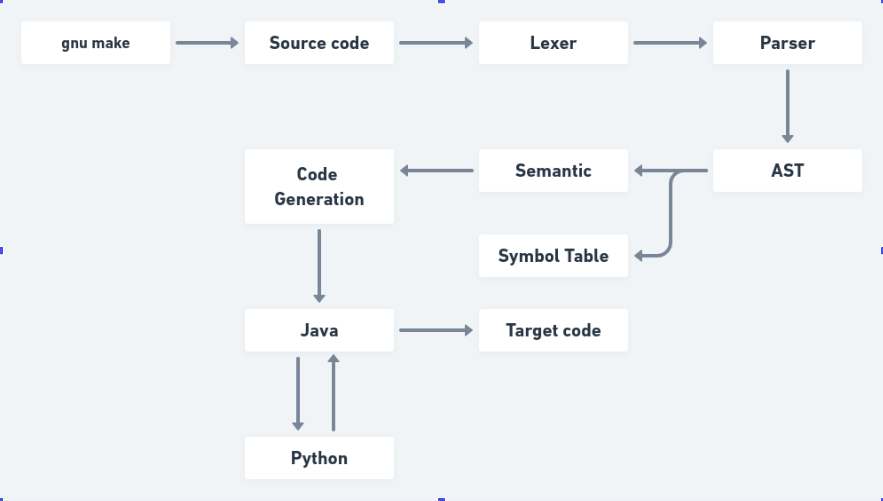
\includegraphics[width=15cm, height =10cm,keepaspectratio]{pictures/Screenshot from 2020-12-18 20-30-12.png}
 \caption{Architecture}
\end{figure}
\section{Lexer}
Stoichy lexer takes input stream from a .sthy program and converts them into tokens. It removes the white spaces and comments in the program. At this stage, errors like invalid characters, incomplete string and incomplete multi line comments are handled. Lexer was written using Ocamllex.

\section{Parser and AST}
Parser takes the tokens generated by the lexer and matches them with grammar rules to form an abstract syntax tree. In parser grammar, there are also exclusive rules for non primitive data types. Some of the non terminals in the grammar are element list ,molecule list.. . Any errors in the syntax will be caught here. Parser was written using Ocamlyacc, hence it is a LALR parser.

\section{Semantic Analysis}
Semantic Analyzer takes the abstract syntax tree generated by the parser, checks if statements and expressions are semantically and syntactically correct. A semantically checked AST is generated. If there are no errors in this stage too, we can use this AST to generate the Java code.

\section{Intermediate code generation}
Most of the code generation is in java and we also used python for balance function in python. Whenever balance function is called, the python script is run and it returns the output to the java console. All the code is put into a java file which contains the Java source code.The generated java code is compiled by javac command in makefile. The primary reason for choosing Java for doing our code generation is as it is machine independent.
\chapter{Development environment}
\section{GNU Make}
  We used \href{https://www.gnu.org/software/make/}{GNU make} as one of the tool as we had many files and many things to compile and \textbf{make} made our work very easy from compiling and converting all the files into objects to cleaning all the intermediaries, \textbf{make} did a very good job. Before knowing about the make file (for first 2 weeks), we used to compile and type each and every command where we used to do a lot of mistakes and hence thought of an alternative, we were amazed by the idea of make and chose to include in our Development environment. The advantages that we learned about make are:
  \begin{itemize}
      \item Make enables the end user to build and install your package without knowing the details of how that is done -- because these details are recorded in the makefile that you supply.
      \item Make figures out automatically which files it needs to update, based on which source files have changed. It also automatically determines the proper order for updating files, in case one non-source file depends on another non-source file.\\ 
      As a result, if you change a few source files and then run Make, it does not need to recompile all of your program. It updates only those non-source files that depend directly or indirectly on the source files that you changed.
      \item GNU Make has many powerful features for use in makefiles, beyond what other Make versions have. It can also regenerate, use, and then delete intermediate files which need not be saved.
  \end{itemize}
  Our final dependency graph looks like the one in the below figure.
 \begin{figure}[H]
 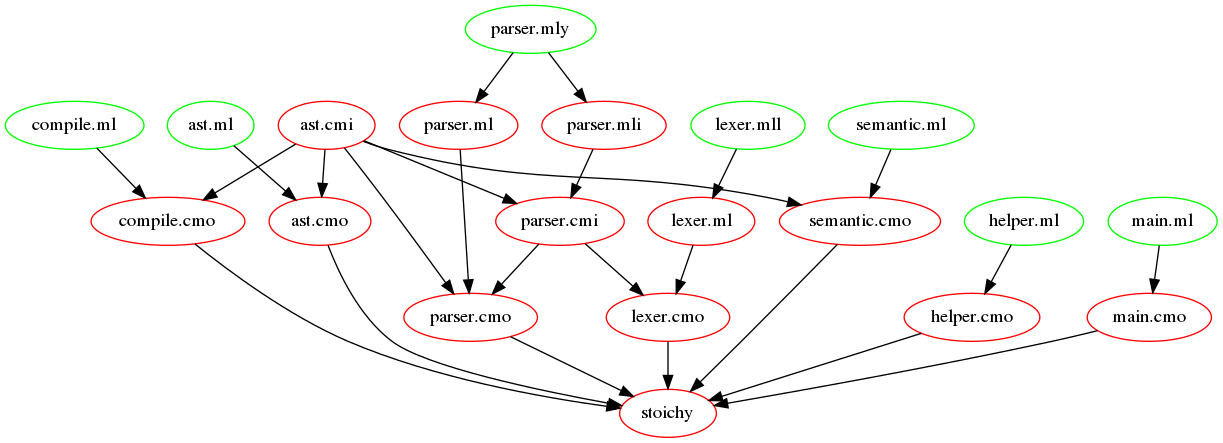
\includegraphics[width=\linewidth,height=\textheight,keepaspectratio]{./pictures/my_graph.png}
 \caption{Makefile Dependencies}
\end{figure}

\section{Bash}
   We used bash as a part of our testing to run and check correctness of all testcases that we wrote.As we used many
  modules and libraries from Ocaml and sympy from python. We had written a bash script where a user can relentlessly just run a bash script and it does it's job of downloading all the required things. 
  
  \section{Git}
    We used Git as our version control system. Where we pushed our work into a remote on GitHub whenever one of us finished working on some feature, we have done some code review and then modified pulled, pushed etc. Our commits are shown in Appendix \ref{Project log} 
    
  \section{VSCode}
   We got into many problems and some of them wanted to be solved at very quickly. All of us Used VSCode particularly \textbf{liveshare} when we ran into problems. We were sometimes successfull in rectiying the mistakes. As VSCode provided liveshare which had many nice featues such as Terminal sharing and Code sharing, syntax highlighting etc, we included it in one of our Tools.

\chapter{Test Plan and Test suites}
    \section{Introduction}
    % Whenever a person makes changes to any of the source code to get an updated version of the the project, we actually can't be very sure that the changes have been made correctly.\newline
    % For solving this problem, 
        We have made a good no. of test cases, which handles all syntax structures (like arithmetic, loops, conditional statements, etc) by running which, we can make sure that the project is in a good state.\\
        % Since there are many test cases to be run and we can't run and check them manually everytime. 
        To be fast and accurate in testing, we have decided to do our testing an automated process. \\ So we have also created expected output files for each test case and had wrote a bash shell script(run\_test.sh), which takes all test cases, executes them and matches the output with the expected output files using the diff command.
        \lstinputlisting[language={},caption={run\_tests.sh bash script}]{run_tests.sh}
    \section{Demo files}
        \lstinputlisting[language={},caption={Hello World test}]{./demo/demofile1.sthy}
        \lstinputlisting[language={},caption={Expected output}]{demo/expected/./demofile1.out}
        
        \lstinputlisting[language={},caption={Methods, Booleans, conditional operators test}]{demo/demofile2.sthy}
        \lstinputlisting[language={},caption={Expected output}]{demo/expected/demofile2.out}
        
        \lstinputlisting[language={},caption={for  and while loops}]{demo/demofile3.sthy}
        \lstinputlisting[language={},caption={Expected output}]{demo/expected/demofile3.out}
        
        \lstinputlisting[language={},caption={Non primitve data types and basic unbuilt functions test}]{demo/demofile4.sthy}
        \lstinputlisting[language={},caption={Expected output}]{demo/expected/demofile4.out}
        
        \lstinputlisting[language={},caption={Main core usage(Balancing of equations) test}]{demo/demofile5.sthy}
        \lstinputlisting[language={},caption={Expected output}]{demo/expected/demofile5.out}
    
    \section{Test cases}
        \lstinputlisting[language={},caption={test1}]{test_cases/test1.sthy}
        \lstinputlisting[language={},caption={Expected output}]{test_cases/expected/test1.out}
        
        \lstinputlisting[language={},caption={test2}]{test_cases/test2.sthy}
        \lstinputlisting[language={},caption={Expected output}]{test_cases/expected/test2.out}
        
        \lstinputlisting[language={},caption={test3}]{test_cases/test3.sthy}
        \lstinputlisting[language={},caption={Expected output}]{test_cases/expected/test3.out}
        
        \lstinputlisting[language={},caption={test4}]{test_cases/test4.sthy}
        \lstinputlisting[language={},caption={Expected output}]{test_cases/expected/test4.out}
        
        \lstinputlisting[language={},caption={test5}]{test_cases/test5.sthy}
        \lstinputlisting[language={},caption={Expected output}]{test_cases/expected/test5.out}
        
        \lstinputlisting[language={},caption={test6}]{test_cases/test6.sthy}
        \lstinputlisting[language={},caption={Expected output}]{test_cases/expected/test6.out}
        
        \lstinputlisting[language={},caption={test7}]{test_cases/test7.sthy}
        \lstinputlisting[language={},caption={Expected output}]{test_cases/expected/test7.out}
        
        \lstinputlisting[language={},caption={test8}]{test_cases/test8.sthy}
        \lstinputlisting[language={},caption={Expected output}]{test_cases/expected/test8.out}
        
        \lstinputlisting[language={},caption={test9}]{test_cases/test9.sthy}
        \lstinputlisting[language={},caption={Expected output}]{test_cases/expected/test9.out}
        
        \lstinputlisting[language={},caption={test10}]{test_cases/test10.sthy}
        \lstinputlisting[language={},caption={Expected output}]{test_cases/expected/test10.out}
        \newpage
    \section{Error cases}
        \lstinputlisting[language={},caption={test8}]{test_cases/errorfiles/test13.sthy}
        
        \lstinputlisting[language={},caption={test9}]{test_cases/errorfiles/test14.sthy}
        
        \lstinputlisting[language={},caption={test10}]{test_cases/errorfiles/test15.sthy}
        
\chapter{Conclusion \& Lessons Learned}

   It was wholly a good experience for us. It firstly weird when we heard that, we didn't know much about all the parts of the compiler along with it we even had to write some new language. Then came the period where sir asked us to form groups and come up with an idea of what we write, i.e a DSL or a compiler or Translator. We felt that it would be very exciting of writing something thoughtown. In first week we searched for so many ideas on what to do. Being inspired from the functional language from POPL course, we thought in that direction. Then we thought of problems we faced in college and all of us where like it would be nice if we do something related to chemical equation calculations. There came the Idea of \textbf{Stoichy}. We started working on it. There were times when we weren't able to debug the code and looked to many blogs and websites such as stackoverflow. Majorly we worked toghether on weekends. As we were a group of 5, arranging time for project was a difficult task.\\ 
   
   \hspace{2cm} As we used Github for version control it became easier to see what others have done and review/modify the code. Our major learnings were about bash scripting, writing make files. Working as a team member was a pretty good experience for all of us. When we were working on balancing function, we thought of doing the code generation in Java and we later realised that it was too lengthy. We started thinking of is there any way to make it simpler. Thats where we learnt about executing the Python code from java by passing the equation as argument. We felt pretty awesome after the Python code was working as it was easier to write in python using its vast linear algebra libraries. Finally we understood about the difficulty in writing a language and design decisions involved in it.
\chapter{Appendix}
\section{Project Log}
\label{Project log}
\lstinputlisting[language={},caption={Project Log from GitHub}]{stoichy_log.txt}
\section{Code Listing}
    All the codes can be found on our Github Page \url{https://github.com/akashtadwai/stoichy}
\end{document}